\documentclass{report}
\usepackage{graphicx}
\begin{document}
    \begin{titlepage}
        \centering
        
        {\bfseries\Huge INTRODUCCIÓN A LA CIENCIA DE DATOS \par}
        \vspace{2cm}
        {
\includegraphics[width= 0.5\textwidth]{CD}\par}
        \vspace{2cm}
        
        {\scshape\large Facultad de Matemática y Computación \par}
        \vspace{3cm}
        {\itshape\large PRESENTACIÓN \par}
        \vspace{3cm}
        {\large Autor: \par}
        {\large Katherine Rodríguez Rodríguez}
    \end{titlepage}
    \begin{center}
        {\underline{\large{INTRODUCCIÓN}}}\\
    \end{center}
    \vspace{2cm}
    \begin{center}
        MYPYMES\\
        $\bullet$Se han insertado poco a poco en el sector económico\\
        $\bullet$Se enfocan en la producción de bienes\\
        $\bullet$En su mayoría son privadas\\
        \vspace{2cm}
        \large{Bienes disponibles}\\
        
        $\swarrow$ \hspace{0,8cm} $\searrow$\\
        Producción Nacional\hspace{0,5cm}Importaciones\\
        $\searrow$\hspace{0,8cm} $\swarrow$\\
        Consumo de hogares, consumo intermedio y exportaciones\\
    \end{center}
    $\bullet$ Las bebidas representan el 85,4 porciento de la producción nacional
    
    \newpage
    \begin{center}
        {\Huge La cebolla}\\
        \vspace{2cm}
        Una visualización mediante un gráfico de barras respecto a la cantidad de lugares donde se vende a un mismo precio, dependiendo del tipo.\\
        \vspace{1cm}
        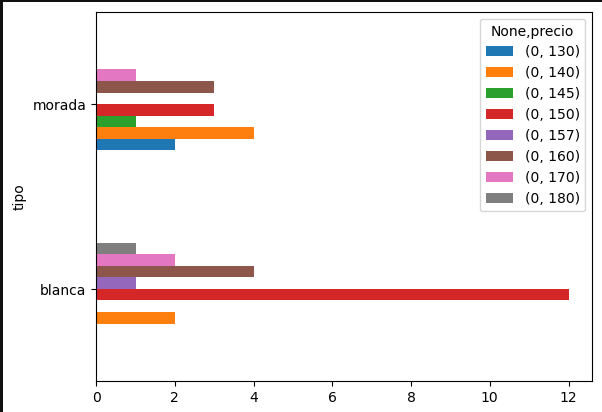
\includegraphics[width= 1.0\textwidth]{c-c-p}\\
    \end{center}
    
    \newpage
    \centering
    El precio dependiendo de el lugar donde se encuentra\\
    \vspace{1cm}
    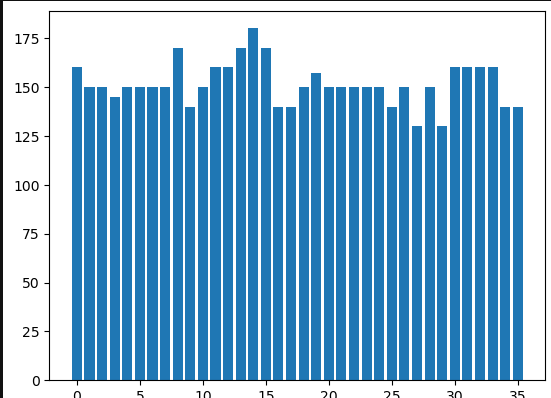
\includegraphics[width= 1.0\textwidth]{barra}\\

    \newpage
    \centering
    {\Huge La cerveza}\\
    \vspace{2cm}
    Cantidad de cervezas dependiendo del tipo de envase\\
    \vspace{1cm}
    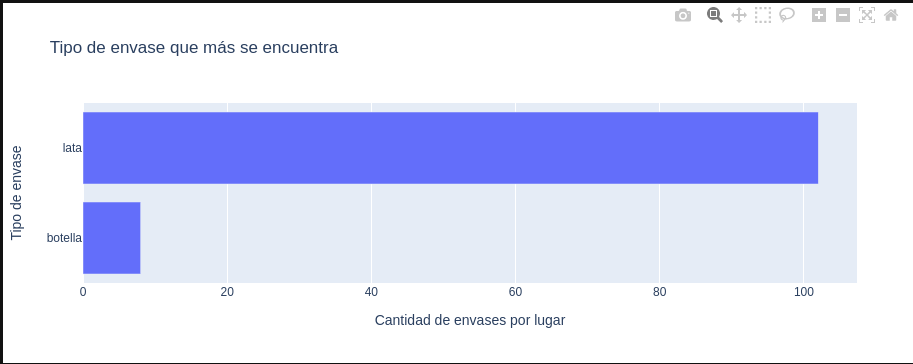
\includegraphics[width= 1.0\textwidth]{envase}\\
    \vspace{1cm}
    Variedad de las cervezas y los diferentes precios que llega a tomar en cada lugar\\
    \vspace{1cm}
    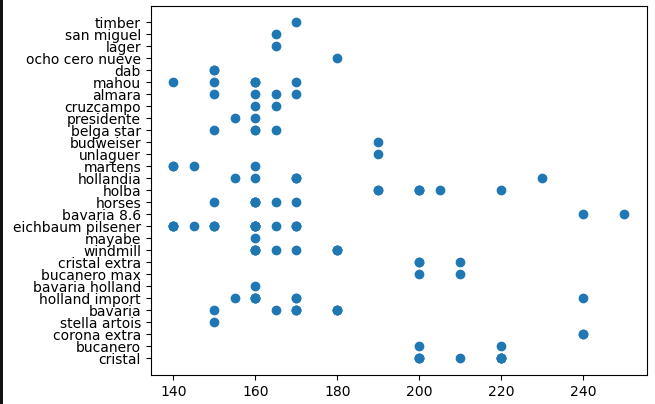
\includegraphics[width= 1.0\textwidth]{cerveza}\\

    \newpage
    \centering
    El tipo de marca que más abunda en el municipio\\
    \vspace{1cm}
    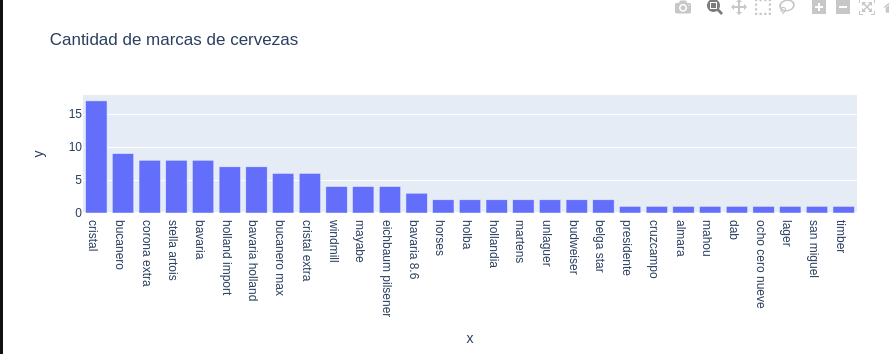
\includegraphics[width= 1.0\textwidth]{+abunda}\\
    
    \newpage
    \centering
    {\Huge La malta}\\
    \vspace{1cm}
    Las diferentes marcas que presenta la malta en los lugares de ventas y sus respectivos precios.\\
    \vspace{1cm}
    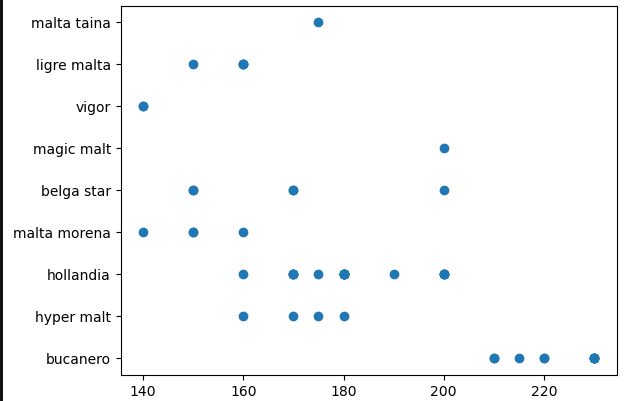
\includegraphics[width= 1.0\textwidth]{malta}\\
    
    \newpage
    La marca que más predomina en el Cotorro\\
    \vspace{1cm}
    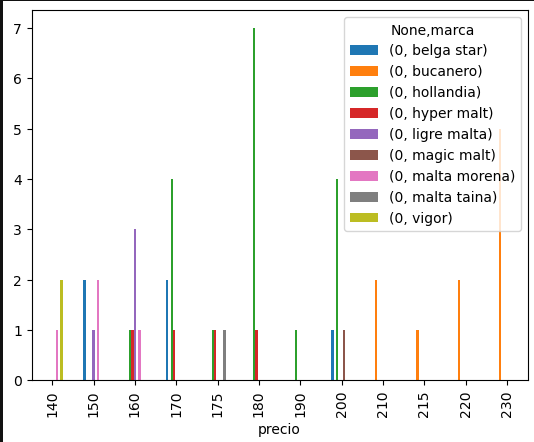
\includegraphics[width= 1.0\textwidth]{m-p}\\
\end{document}

